% Options for packages loaded elsewhere
\PassOptionsToPackage{unicode}{hyperref}
\PassOptionsToPackage{hyphens}{url}
\documentclass[
  12pt,
]{article}
\usepackage{xcolor}
\usepackage[margin=1in]{geometry}
\usepackage{amsmath,amssymb}
\setcounter{secnumdepth}{5}
\usepackage{iftex}
\ifPDFTeX
  \usepackage[T1]{fontenc}
  \usepackage[utf8]{inputenc}
  \usepackage{textcomp} % provide euro and other symbols
\else % if luatex or xetex
  \usepackage{unicode-math} % this also loads fontspec
  \defaultfontfeatures{Scale=MatchLowercase}
  \defaultfontfeatures[\rmfamily]{Ligatures=TeX,Scale=1}
\fi
\usepackage{lmodern}
\ifPDFTeX\else
  % xetex/luatex font selection
\fi
% Use upquote if available, for straight quotes in verbatim environments
\IfFileExists{upquote.sty}{\usepackage{upquote}}{}
\IfFileExists{microtype.sty}{% use microtype if available
  \usepackage[]{microtype}
  \UseMicrotypeSet[protrusion]{basicmath} % disable protrusion for tt fonts
}{}
\makeatletter
\@ifundefined{KOMAClassName}{% if non-KOMA class
  \IfFileExists{parskip.sty}{%
    \usepackage{parskip}
  }{% else
    \setlength{\parindent}{0pt}
    \setlength{\parskip}{6pt plus 2pt minus 1pt}}
}{% if KOMA class
  \KOMAoptions{parskip=half}}
\makeatother
\usepackage{longtable,booktabs,array}
\usepackage{calc} % for calculating minipage widths
% Correct order of tables after \paragraph or \subparagraph
\usepackage{etoolbox}
\makeatletter
\patchcmd\longtable{\par}{\if@noskipsec\mbox{}\fi\par}{}{}
\makeatother
% Allow footnotes in longtable head/foot
\IfFileExists{footnotehyper.sty}{\usepackage{footnotehyper}}{\usepackage{footnote}}
\makesavenoteenv{longtable}
\usepackage{graphicx}
\makeatletter
\newsavebox\pandoc@box
\newcommand*\pandocbounded[1]{% scales image to fit in text height/width
  \sbox\pandoc@box{#1}%
  \Gscale@div\@tempa{\textheight}{\dimexpr\ht\pandoc@box+\dp\pandoc@box\relax}%
  \Gscale@div\@tempb{\linewidth}{\wd\pandoc@box}%
  \ifdim\@tempb\p@<\@tempa\p@\let\@tempa\@tempb\fi% select the smaller of both
  \ifdim\@tempa\p@<\p@\scalebox{\@tempa}{\usebox\pandoc@box}%
  \else\usebox{\pandoc@box}%
  \fi%
}
% Set default figure placement to htbp
\def\fps@figure{htbp}
\makeatother
\setlength{\emergencystretch}{3em} % prevent overfull lines
\providecommand{\tightlist}{%
  \setlength{\itemsep}{0pt}\setlength{\parskip}{0pt}}
\usepackage{setspace}
\AtBeginDocument{\let\maketitle\relax}
\usepackage{bookmark}
\IfFileExists{xurl.sty}{\usepackage{xurl}}{} % add URL line breaks if available
\urlstyle{same}
\hypersetup{
  pdftitle={ROSSMANN STORE TYPE A SALES FORECASTING REPORT},
  pdfauthor={Samin Intisar, Jensen Suhenda, Shannon Sulistio, Yolanda Wu, Huaxi Zeng},
  hidelinks,
  pdfcreator={LaTeX via pandoc}}

\title{ROSSMANN STORE TYPE A SALES FORECASTING REPORT}
\author{Samin Intisar, Jensen Suhenda, Shannon Sulistio, Yolanda Wu,
Huaxi Zeng}
\date{April 2026}

\begin{document}
\maketitle

\begin{titlepage}
\centering
\vspace*{2.5cm}
{\LARGE \bfseries ROSSMANN STORE TYPE A SALES FORECASTING \par}
\vspace{2cm}
{\Large STAT 443 - Time Series \& Forecasting \par}
\vspace{1.5cm}
{\large
Yolanda Wu\par
Samin Intisar\par
Shannon Sulistio\par
Yolanda Wu\par
Huaxi Zeng\par
}
\vfill
{\large Department of Statistics\par
University of British Columbia\par
Vancouver, BC, Canada\par
April 2026\par}
\end{titlepage}
\tableofcontents
\newpage

\section{Abstract}\label{abstract}

\subsection{Project Goal}\label{project-goal}

The goal of this project is to forecast aggregate daily Rossmann store
sales and evaluate which time series forecasting method provides the
most accurate predictions over a six-week forecasting horizon. The main
research question is: Which forecasting model best predicts Rossmann
daily sales among simple rules, exponential smoothing, ARIMA, and
ARMAX/ARIMAX methods?

The motivation for this project is that accurate sales forecasting is
important for retail businesses because it can improve staffing
decisions, inventory planning, and promotional management. Since
Rossmann sales exhibit strong seasonal and operational patterns,
forecasting models may help better capture these dynamics.

\subsection{Project Outcome}\label{project-outcome}

Our results suggest that simple rules such as persistence and average
forecasts provide reasonable baseline predictions but have limited
flexibility. Exponential smoothing improves forecasting performance by
capturing weekly seasonal patterns in the sales data. ARIMA models
further improve predictions by accounting for autocorrelation in the
time series. Among all methods considered, ARMAX/ARIMAX models achieve
the best forecasting performance, indicating that including explanatory
variables improves prediction accuracy beyond purely time-series-based
models.

\section{Data Description}\label{data-description}

\subsection{Data Collection and Scope}\label{data-collection-and-scope}

\textbf{Data Source:}
\href{https://www.kaggle.com/c/rossmann-store-sales/data}{Rossmann Store
Sales \textbar{} Kaggle} \textbf{Project Repository:}
\href{https://github.com/samintisar/stat443-timeseries-project}{GitHub
Repo}

We are provided with historical sales data for 1,115 Rossmann stores.
The original Rossmann setup is row-level Sales prediction for the test
set, but this project intentionally narrows scope to
\textbf{aggregate-daily Sales for Store Type A}. Note that some stores
in the dataset were temporarily closed for refurbishment.

\subsubsection{Raw Datasets}\label{raw-datasets}

\begin{itemize}
\tightlist
\item
  \texttt{train.csv} - historical data including Sales
\item
  \texttt{test.csv} - historical data excluding Sales
\item
  \texttt{sample\_submission.csv} - original row-level competition
  format (reference only for this project)
\item
  \texttt{store.csv} - supplemental information about the stores
\end{itemize}

\subsubsection{Data Fields}\label{data-fields}

Most of the fields are self-explanatory. The following are descriptions
for those that aren't:

\begin{itemize}
\tightlist
\item
  \textbf{Id} - an Id that represents a (Store, Date) duple within the
  test set (not the final prediction unit in this project)
\item
  \textbf{Store} - a unique Id for each store
\item
  \textbf{Sales} - the turnover for any given day; this project predicts
  the \textbf{sum of Sales across Store Type A per date}
\item
  \textbf{Customers} - the number of customers on a given day
\item
  \textbf{Open} - an indicator for whether the store was open: 0 =
  closed, 1 = open
\item
  \textbf{StateHoliday} - indicates a state holiday. Normally all
  stores, with few exceptions, are closed on state holidays. Note that
  all schools are closed on public holidays and weekends. a = public
  holiday, b = Easter holiday, c = Christmas, 0 = None
\item
  \textbf{SchoolHoliday} - indicates if the (Store, Date) was affected
  by the closure of public schools
\item
  \textbf{StoreType} - differentiates between 4 different store models:
  a, b, c, d
\item
  \textbf{Assortment} - describes an assortment level: a = basic, b =
  extra, c = extended
\item
  \textbf{CompetitionDistance} - distance in meters to the nearest
  competitor store
\item
  \textbf{CompetitionOpenSince{[}Month/Year{]}} - gives the approximate
  year and month of the time the nearest competitor was opened
\item
  \textbf{Promo} - indicates whether a store is running a promo on that
  day
\item
  \textbf{Promo2} - Promo2 is a continuing and consecutive promotion for
  some stores: 0 = store is not participating, 1 = store is
  participating
\item
  \textbf{Promo2Since{[}Year/Week{]}} - describes the year and calendar
  week when the store started participating in Promo2
\item
  \textbf{PromoInterval} - describes the consecutive intervals Promo2 is
  started, naming the months the promotion is started anew. E.g.
  ``Feb,May,Aug,Nov'' means each round starts in February, May, August,
  November of any given year for that store
\end{itemize}

\subsection{Data Wrangling Pipeline}\label{data-wrangling-pipeline}

The raw Rossmann dataset consists of daily sales records for individual
stores along with store-level attributes. Since our analysis focuses on
aggregate daily sales for Store Type ``a'', the data was preprocessed to
create a consistent time series suitable for modeling.

First, the \texttt{train} and \texttt{store} datasets were merged using
the \texttt{Store} identifier to combine sales information with store
characteristics. The data was then filtered to include only Store Type
``a'', ensuring consistency across all subsequent analyses.

Next, the data was aggregated to the daily level by summing sales across
all relevant stores for each date. This produced a univariate time
series where each observation represents total daily sales across Store
Type ``a''.

To ensure a valid time series structure, the dataset was arranged in
chronological order and missing dates were filled to create a continuous
daily sequence. This step is important for time series models such as
ARIMA, which assume evenly spaced observations.

In addition to the aggregated sales series, we created two versions of
the processed dataset:

\begin{itemize}
\tightlist
\item
  A clean univariate dataset, containing only daily sales and time
  indices, used for baseline time series models such as ARIMA and
  exponential smoothing.
\item
  An extended dataset, which includes additional explanatory variables
  such as promotion and holiday indicators. These variables were
  aggregated as proportions across stores (for example, proportion of
  stores running promotions on a given day) to capture external factors
  that may influence sales. We also included calendar-based features
  like \texttt{DayOfWeek} and \texttt{IsWeekend} to capture temporal
  patterns in the data.
\end{itemize}

Finally, all processed datasets were saved to a shared directory to
ensure that all team members used a consistent input for modeling and
evaluation.

Table 3 shows a preview of the processed dataset
(\texttt{store\_type\_a\_train\_aggregate\_daily.csv}), which serves as
the main input for the time series analysis.

\begin{longtable}[]{@{}
  >{\raggedright\arraybackslash}p{(\linewidth - 14\tabcolsep) * \real{0.1719}}
  >{\raggedleft\arraybackslash}p{(\linewidth - 14\tabcolsep) * \real{0.1250}}
  >{\raggedleft\arraybackslash}p{(\linewidth - 14\tabcolsep) * \real{0.0781}}
  >{\raggedleft\arraybackslash}p{(\linewidth - 14\tabcolsep) * \real{0.1406}}
  >{\raggedleft\arraybackslash}p{(\linewidth - 14\tabcolsep) * \real{0.2031}}
  >{\raggedleft\arraybackslash}p{(\linewidth - 14\tabcolsep) * \real{0.0625}}
  >{\raggedleft\arraybackslash}p{(\linewidth - 14\tabcolsep) * \real{0.0938}}
  >{\raggedleft\arraybackslash}p{(\linewidth - 14\tabcolsep) * \real{0.1250}}@{}}
\caption{Preview of processed dataset
(store\_type\_a\_train\_aggregate\_daily.csv).}\tabularnewline
\toprule\noalign{}
\begin{minipage}[b]{\linewidth}\raggedright
Date
\end{minipage} & \begin{minipage}[b]{\linewidth}\raggedleft
Sales
\end{minipage} & \begin{minipage}[b]{\linewidth}\raggedleft
Open
\end{minipage} & \begin{minipage}[b]{\linewidth}\raggedleft
PromoPct
\end{minipage} & \begin{minipage}[b]{\linewidth}\raggedleft
SchoolHolPct
\end{minipage} & \begin{minipage}[b]{\linewidth}\raggedleft
DOW
\end{minipage} & \begin{minipage}[b]{\linewidth}\raggedleft
Month
\end{minipage} & \begin{minipage}[b]{\linewidth}\raggedleft
Weekend
\end{minipage} \\
\midrule\noalign{}
\endfirsthead
\toprule\noalign{}
\begin{minipage}[b]{\linewidth}\raggedright
Date
\end{minipage} & \begin{minipage}[b]{\linewidth}\raggedleft
Sales
\end{minipage} & \begin{minipage}[b]{\linewidth}\raggedleft
Open
\end{minipage} & \begin{minipage}[b]{\linewidth}\raggedleft
PromoPct
\end{minipage} & \begin{minipage}[b]{\linewidth}\raggedleft
SchoolHolPct
\end{minipage} & \begin{minipage}[b]{\linewidth}\raggedleft
DOW
\end{minipage} & \begin{minipage}[b]{\linewidth}\raggedleft
Month
\end{minipage} & \begin{minipage}[b]{\linewidth}\raggedleft
Weekend
\end{minipage} \\
\midrule\noalign{}
\endhead
\bottomrule\noalign{}
\endlastfoot
2013-01-01 & 2907 & 1 & 0 & 1.000 & 2 & 1 & 0 \\
2013-01-02 & 3920386 & 602 & 0 & 1.000 & 3 & 1 & 0 \\
2013-01-03 & 3528027 & 601 & 0 & 0.939 & 4 & 1 & 0 \\
2013-01-04 & 3610215 & 601 & 0 & 0.939 & 5 & 1 & 0 \\
2013-01-05 & 2964587 & 600 & 0 & 0.066 & 6 & 1 & 1 \\
2013-01-06 & 6254 & 3 & 0 & 0.066 & 7 & 1 & 1 \\
\end{longtable}

\subsection{Exploratory Data Analysis
(EDA)}\label{exploratory-data-analysis-eda}

We are doing an Exploratory Data Analysis on Store Type ``a''. Here are
the key questions we consider to justify modeling choices later in the
report:

\begin{itemize}
\tightlist
\item
  What does the sales data look like? Is it stable, trending up/down, or
  highly volatile?
\item
  Is there a pattern? Do sales repeat weekly or monthly?
\item
  What affects sales? Do promo, competition, and day-of-week matter?
\item
  Is the series stationary? This informs ARIMA differencing choices.
\end{itemize}

\subsubsection{Variables used in EDA}\label{variables-used-in-eda}

The EDA primarily uses the processed training datasets:

\begin{itemize}
\tightlist
\item
  \texttt{Date}: calendar date for each daily observation.
\item
  \texttt{Sales}: aggregate daily sales across all Store Type ``a''
  stores (main response series).
\item
  \texttt{PromoShare}: proportion of stores with active promotions on a
  given date.
\item
  \texttt{OpenStores}: number of open Store Type ``a'' stores on each
  date.
\item
  \texttt{SchoolHolidayShare}: proportion of stores affected by school
  holidays.
\item
  \texttt{DayOfWeek}, \texttt{Month}, \texttt{IsoWeek},
  \texttt{IsWeekend}: calendar variables used to assess recurring
  patterns.
\item
  \texttt{CompetitionDistance} (from store-level processed data): used
  for the competition-sales relationship check.
\end{itemize}

\subsubsection{Summary of data}\label{summary-of-data}

Basic statistics of aggregated daily sales across all stores help us
understand the range and distribution of sales.

\begin{longtable}[]{@{}lr@{}}
\caption{Summary statistics for aggregate daily sales (Store Type
a).}\tabularnewline
\toprule\noalign{}
Statistic & Value \\
\midrule\noalign{}
\endfirsthead
\toprule\noalign{}
Statistic & Value \\
\midrule\noalign{}
\endhead
\bottomrule\noalign{}
\endlastfoot
Min. & 0 \\
1st Qu. & 2994007 \\
Median & 3563651 \\
Mean & 3360228 \\
3rd Qu. & 4459143 \\
Max. & 8511488 \\
\end{longtable}

Based on Figure 2.1, daily total sales for Store Type ``a'' range from
680 to about 8.5 million, with a median around 3.6 million and mean
around 3.5 million. Since the mean and median are very close, the
distribution appears fairly symmetric. The minimum value (680) is very
low and likely corresponds to a day where almost all Type ``a'' stores
were closed.

\subsubsection{Date continuity check}\label{date-continuity-check}

This check was included in the original EDA file and confirms the daily
series is complete over the observed range.

\begin{longtable}[]{@{}llrrr@{}}
\caption{Date continuity check for aggregate daily
series.}\tabularnewline
\toprule\noalign{}
first\_date & last\_date & expected\_days & observed\_days &
missing\_days \\
\midrule\noalign{}
\endfirsthead
\toprule\noalign{}
first\_date & last\_date & expected\_days & observed\_days &
missing\_days \\
\midrule\noalign{}
\endhead
\bottomrule\noalign{}
\endlastfoot
2013-01-01 & 2015-07-31 & 942 & 942 & 0 \\
\end{longtable}

\subsubsection{Plot of total daily sales for Store Type ``a'' over
dates}\label{plot-of-total-daily-sales-for-store-type-a-over-dates}

We want to understand whether there is trend, visible seasonality, and
potential outliers.

\pandocbounded{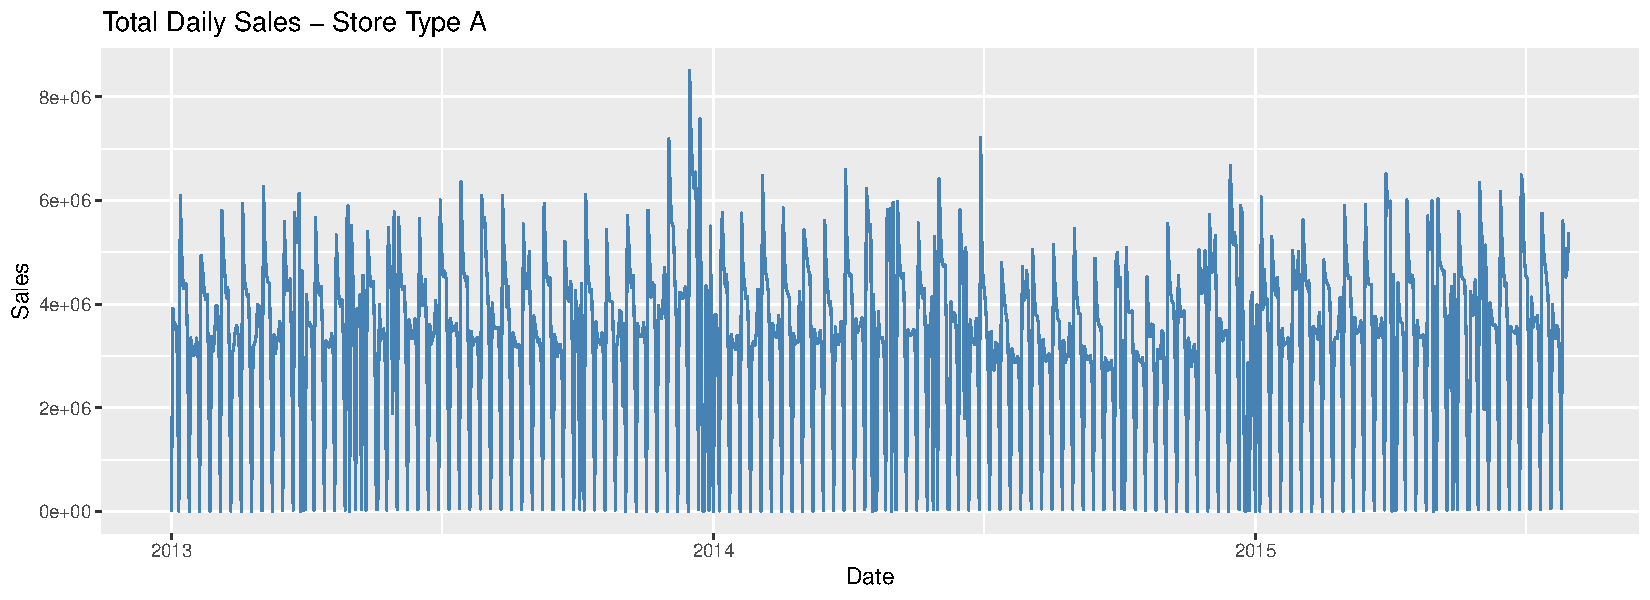
\includegraphics[keepaspectratio]{report_files/report_files/figure-latex/eda-sales-series-1.pdf}}

Based on Figure 2.2, we observe:

\begin{itemize}
\tightlist
\item
  Strong weekly seasonality, with repeating spikes and dips throughout
  the series.
\item
  No clear long-run upward or downward trend; overall level appears
  relatively stable across 2013 to 2015.
\item
  Some outlier spikes around early 2014, potentially linked to holidays
  or special events.
\item
  Some near-zero drops, likely corresponding to Sundays or holidays when
  most stores were closed.
\end{itemize}

\subsubsection{Compare average sales of Store Type ``a'' on promo vs
non-promo
days}\label{compare-average-sales-of-store-type-a-on-promo-vs-non-promo-days}

If mean sales are higher on promo days, this supports including
promotion signals in later ARMAX models.

\begin{longtable}[]{@{}rrr@{}}
\caption{Average daily sales on promo vs non-promo days (PromoDay: 1 =
promo, 0 = non-promo).}\tabularnewline
\toprule\noalign{}
PromoDay & mean\_sales & sd\_sales \\
\midrule\noalign{}
\endfirsthead
\toprule\noalign{}
PromoDay & mean\_sales & sd\_sales \\
\midrule\noalign{}
\endhead
\bottomrule\noalign{}
\endlastfoot
0 & 2507644 & 1554217 \\
1 & 4757320 & 949401 \\
\end{longtable}

From Figure 2.3, non-promo days have substantially lower mean sales than
promo days, with promo-day mean sales being close to double in
magnitude. This supports including promotion-related predictors in the
ARMAX specification.

\subsubsection{Day-of-week effect}\label{day-of-week-effect}

\pandocbounded{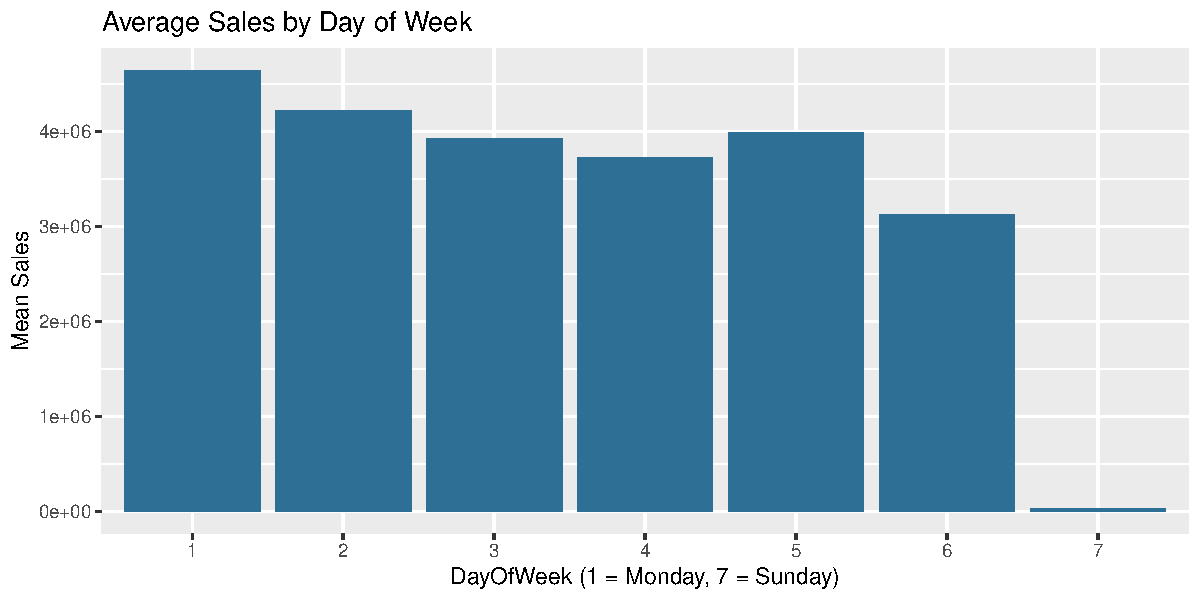
\includegraphics[keepaspectratio]{report_files/report_files/figure-latex/eda-day-of-week-1.pdf}}

\subsubsection{Scatter plot of competition distance vs mean sales for
Store Type
``a''}\label{scatter-plot-of-competition-distance-vs-mean-sales-for-store-type-a}

\pandocbounded{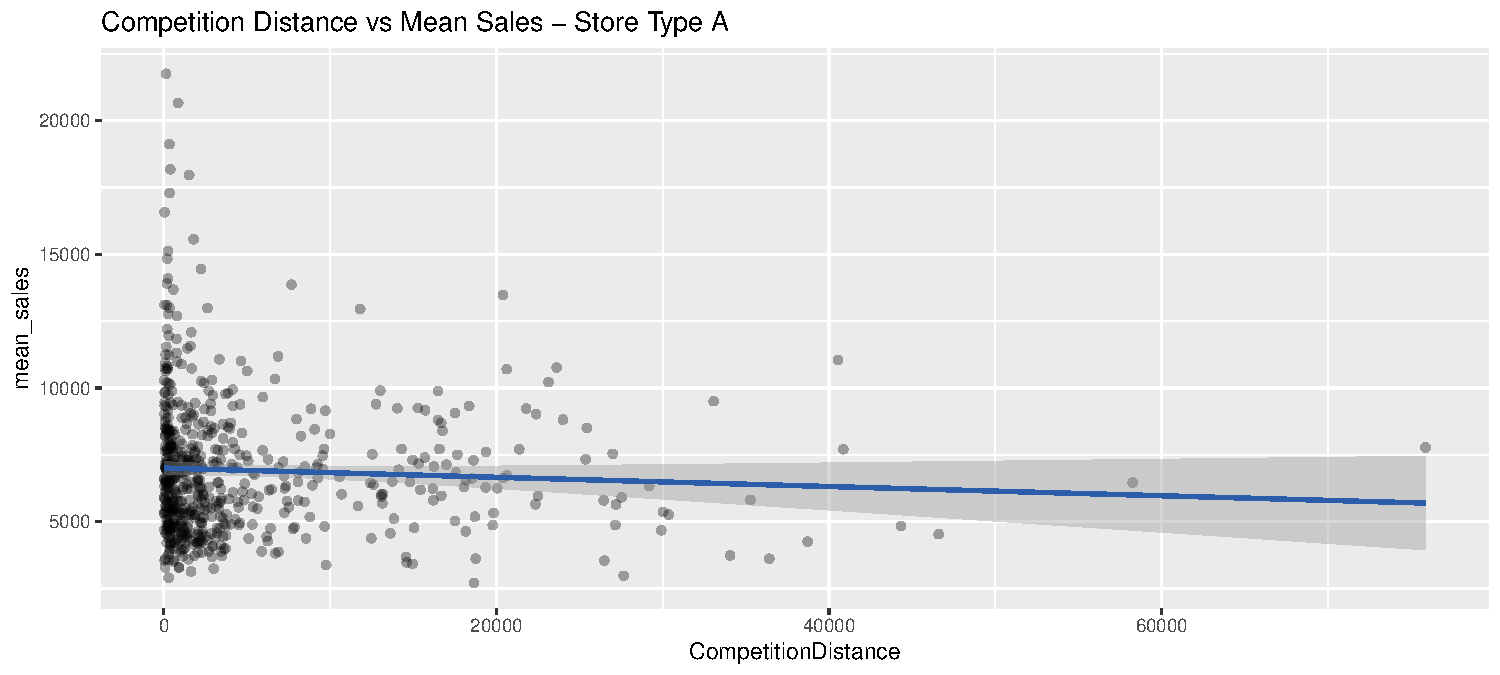
\includegraphics[keepaspectratio]{report_files/report_files/figure-latex/eda-competition-distance-1.pdf}}

As shown in Figure 2.4, the fitted line slopes downward, suggesting a
negative relationship between competition distance and mean sales. The
relationship appears weak because points are widely dispersed, so
\texttt{CompetitionDistance} is likely a marginal explanatory feature
rather than a dominant driver.

\subsubsection{ACF and PACF plots for Store Type
``a''}\label{acf-and-pacf-plots-for-store-type-a}

ACF shows how correlated today's sales are with values from previous
days. Spikes at lags 7, 14, 21, and 28 indicate weekly seasonality.

\pandocbounded{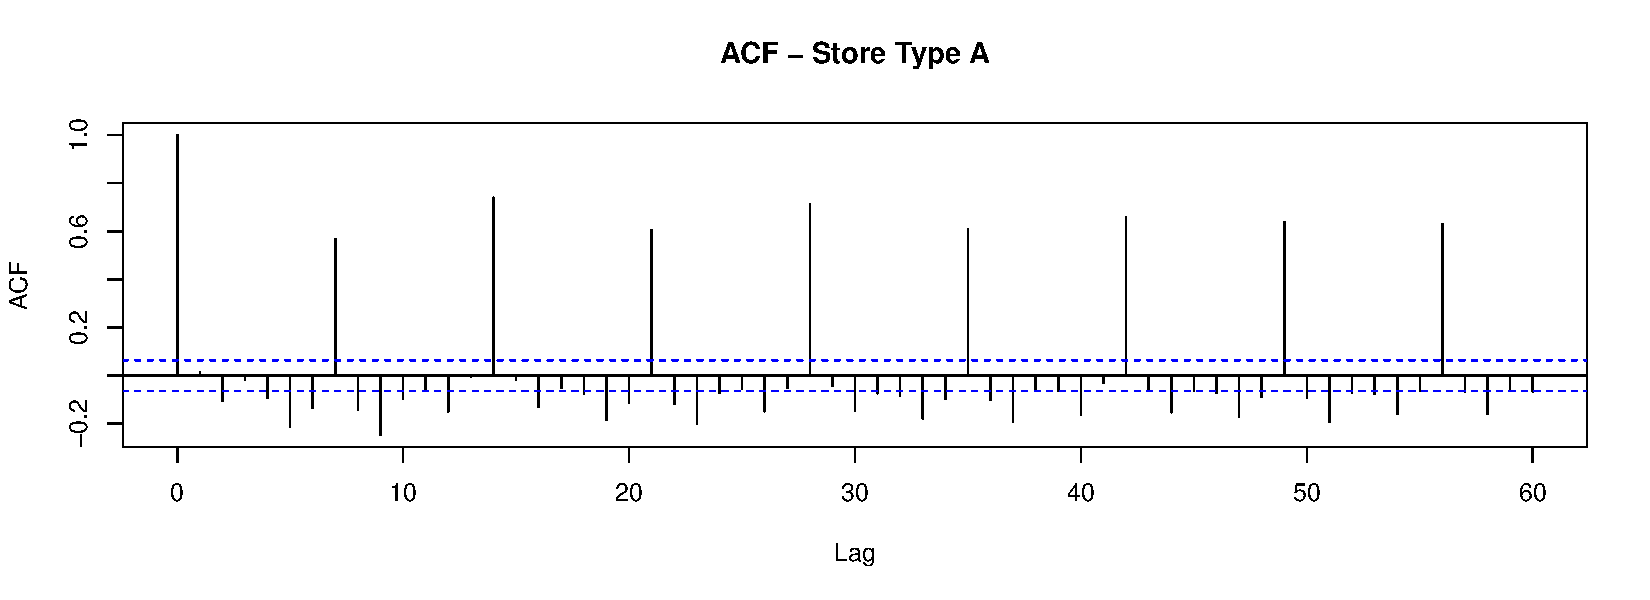
\includegraphics[keepaspectratio]{report_files/report_files/figure-latex/eda-acf-1.pdf}}

In Figure 2.5.1, clear spikes at multiples of 7 confirm strong weekly
seasonality. This supports a seasonal ARIMA component with period 7.

PACF shows partial correlation at each lag after accounting for shorter
lags, which helps identify AR order.

\pandocbounded{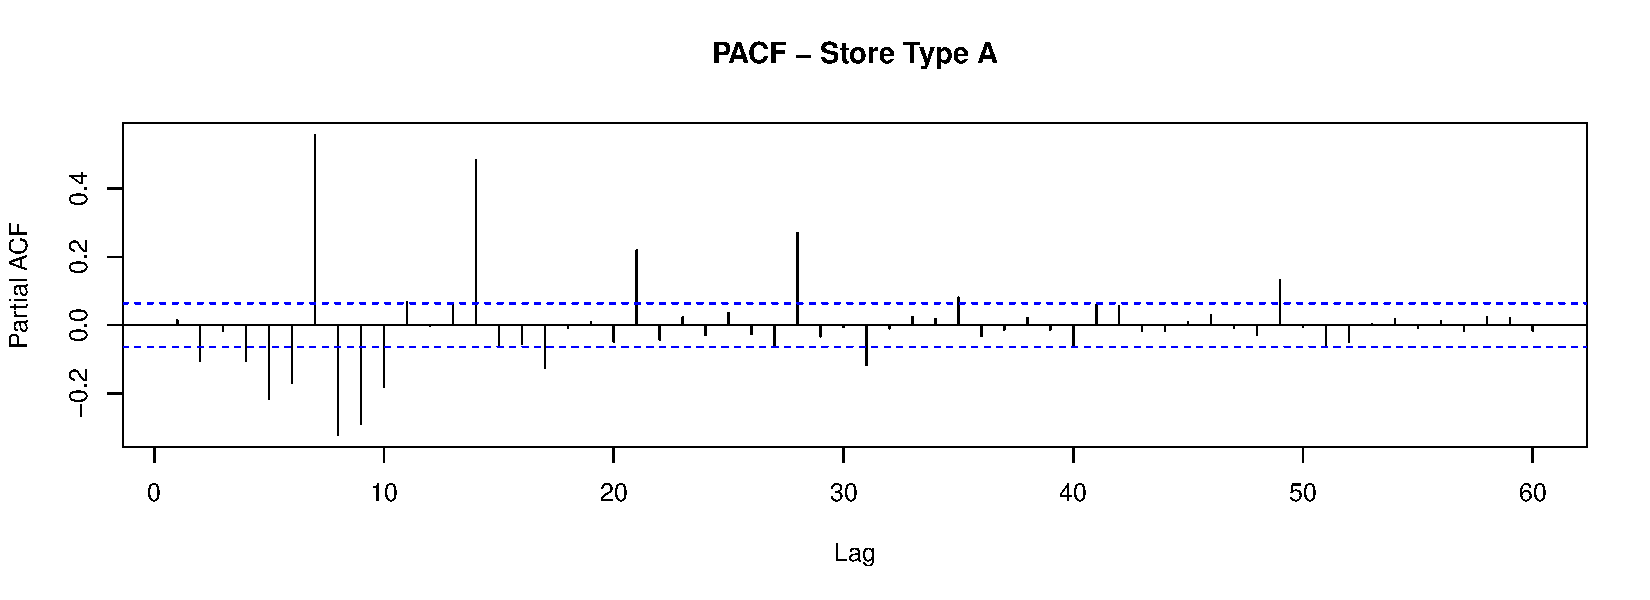
\includegraphics[keepaspectratio]{report_files/report_files/figure-latex/eda-pacf-1.pdf}}

In Figure 2.5.2, notable spikes around seasonal lags (for example 7 and
14), with most other lags within confidence bounds, suggest a low-order
seasonal AR structure is reasonable for ARIMA candidates.

\subsubsection{STL decomposition}\label{stl-decomposition}

STL splits the series into three components:

\begin{enumerate}
\def\labelenumi{\arabic{enumi}.}
\tightlist
\item
  Trend: long-term direction.
\item
  Seasonal: repeating weekly pattern.
\item
  Remainder: what is left after removing trend and seasonality.
\end{enumerate}

\pandocbounded{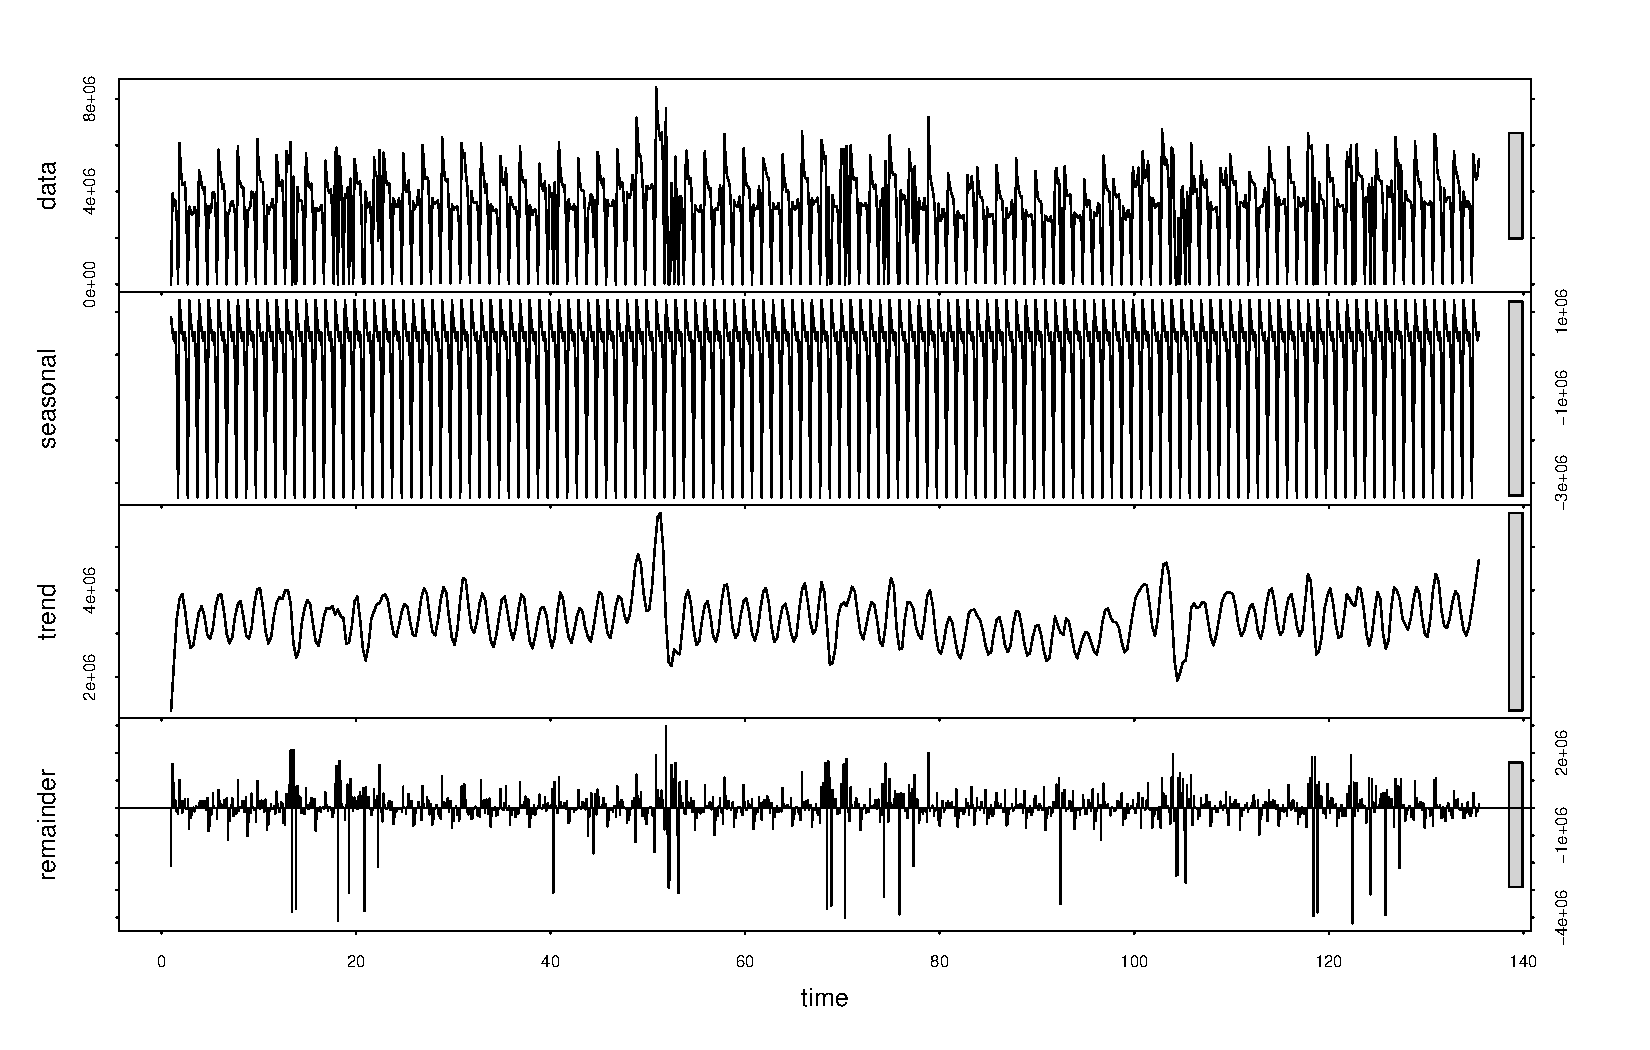
\includegraphics[keepaspectratio]{report_files/report_files/figure-latex/eda-stl-1.pdf}}

Based on Figure 2.6:

\begin{itemize}
\tightlist
\item
  Data: raw series with full variation.
\item
  Trend: relatively flat overall, with a noticeable spike around early
  2014.
\item
  Seasonal: strong, consistent weekly pattern across the full period.
\item
  Remainder: mostly noise around zero with a few larger spikes.
\end{itemize}

\subsubsection{Augmented Dickey-Fuller and KPSS
test}\label{augmented-dickey-fuller-and-kpss-test}

ADF tests stationarity with null hypothesis of non-stationarity:

\begin{itemize}
\tightlist
\item
  \(p < 0.05\): stationary.
\item
  \(p > 0.05\): non-stationary.
\end{itemize}

KPSS is interpreted in the opposite direction:

\begin{itemize}
\tightlist
\item
  \(p > 0.05\): stationary.
\item
  \(p < 0.05\): non-stationary.
\end{itemize}

\begin{longtable}[]{@{}lrrl@{}}
\caption{Stationarity test summary for aggregate daily
sales.}\tabularnewline
\toprule\noalign{}
Test & Statistic & p-value & Decision \\
\midrule\noalign{}
\endfirsthead
\toprule\noalign{}
Test & Statistic & p-value & Decision \\
\midrule\noalign{}
\endhead
\bottomrule\noalign{}
\endlastfoot
ADF & -15.968 & 0.01 & Stationary (reject H0) \\
KPSS & 0.126 & 0.10 & Stationary (fail to reject H0) \\
\end{longtable}

The stationarity test summary shows that ADF supports stationarity while
KPSS also supports stationarity under its opposite null definition.
Since both tests align, a non-seasonal differencing order of \(d = 0\)
is a reasonable starting point for ARIMA candidates.

\subsubsection{EDA implications for
modeling}\label{eda-implications-for-modeling}

To preserve key points from the original EDA file, we summarize the
direct implications:

\begin{itemize}
\tightlist
\item
  Strong weekly behavior supports seasonal terms with period 7.
\item
  Promotion and calendar effects support including exogenous regressors
  in ARMAX.
\item
  Stationarity diagnostics suggest limited need for non-seasonal
  differencing.
\end{itemize}

\section{Methods}\label{methods}

\subsection{Simple Rules Baselines}\label{simple-rules-baselines}

We compare four aggregate-daily baseline forecasts for Store Type A
using a common chronological 80/20 holdout split (first 80\% train, last
20\% holdout): global average, persistence (last observation),
persistence by period (same day previous week), and IID by period
(historical mean for the same day-of-week). Holdout predictions are
generated for each method and evaluated with RMSE to establish benchmark
performance before moving to more complex models.

\subsection{Exponential Smoothing
(ETS)}\label{exponential-smoothing-ets}

Exponential smoothing is fit on the same training subset as above, with
weekly frequency (\(m=7\)). We evaluate both a direct ETS model and an
STL+ETS alternative on the same holdout horizon, then compare holdout
RMSE. This framework tests whether explicit seasonal decomposition
improves forecasts relative to a direct ETS specification for the
aggregate daily series.

\subsection{ARIMA}\label{arima}

ARIMA modeling starts with automated identification using
\texttt{auto.arima} on the aggregate daily series (weekly seasonality).
Because the lowest-AIC model is not always the best forecasting model,
we also fit alternative candidate specifications motivated by residual
diagnostics, especially remaining seasonal autocorrelation at lags near
multiples of 7. Candidate models are compared by AIC, and residual
checks (ACF behavior, distribution shape, and Ljung-Box test) are used
to assess whether residuals are close to white noise.

\subsection{ARMAX}\label{armax}

ARMAX extends ARIMA by including exogenous predictors constructed in
wrangling and EDA: \texttt{PromoShare}, \texttt{OpenStores}, and
calendar effects (\texttt{DayOfWeek}, \texttt{Month}). Using the same
chronological holdout split, we define multiple candidate formulas of
increasing complexity, fit each model on the training set, and use train
AIC as an initial filter. The selected specification is then evaluated
with fixed-coefficient 1-step holdout forecasts and RMSE, followed by
residual diagnostics; finally, the best ARMAX model is refit on full
training data to produce aggregate-daily test forecasts.

\section{Results}\label{results}

\subsection{Holdout Evaluation Design}\label{holdout-evaluation-design}

All candidate methods are evaluated using the same chronological 80/20
split on the aggregate Store Type A training series: the first 80\% of
days are used for model fitting and the final 20\% are held out for
evaluation. This produces a common holdout of 189 observations, so RMSE
comparisons are on the same time window across methods.

To keep comparison fairness, ETS RMSE is recomputed on this same 189-day
holdout in this report (rather than using earlier intermediate output
computed on a shorter window).

The main limitation is that this is a single holdout split rather than
rolling-origin cross-validation, so results are sensitive to this
specific split date. In addition, the provided aggregate test feature
file has no \texttt{Sales} column, so true test RMSE cannot be computed
from that file.

\subsection{RMSE Comparison Across
Methods}\label{rmse-comparison-across-methods}

Table 4.2 compares holdout RMSE across Simple Rules, ETS, ARIMA, and
ARMAX under the same 189-day holdout window.

\begin{longtable}[]{@{}llrr@{}}
\caption{Holdout RMSE comparison across finalized methods (common
holdout window).}\tabularnewline
\toprule\noalign{}
method & model & holdout\_rmse & n\_holdout \\
\midrule\noalign{}
\endfirsthead
\toprule\noalign{}
method & model & holdout\_rmse & n\_holdout \\
\midrule\noalign{}
\endhead
\bottomrule\noalign{}
\endlastfoot
ARMAX & ARMAX\_Promo\_Open\_DOW\_Month & 399947.5 & 189 \\
Simple & iid\_by\_period & 1013538.2 & 189 \\
ARIMA & ARIMA\_m2 & 1016497.2 & 189 \\
ETS & ETS & 1042205.4 & 189 \\
Simple & persistence\_by\_period & 1665219.2 & 189 \\
Simple & global\_average & 1784744.4 & 189 \\
Simple & persistence & 2516853.2 & 189 \\
\end{longtable}

\pandocbounded{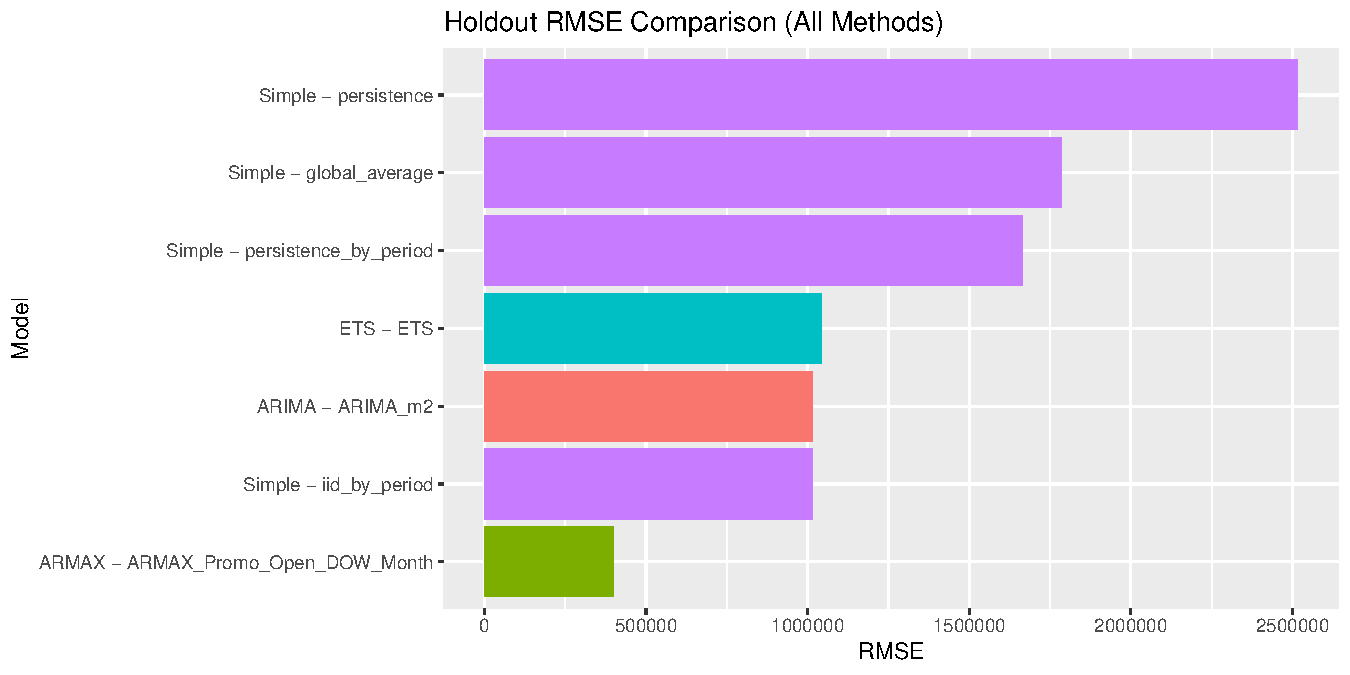
\includegraphics[keepaspectratio]{report_files/report_files/figure-latex/results-rmse-plot-1.pdf}}

ARMAX substantially outperforms all other methods and is the clear
best-performing approach in this comparison. The size of this RMSE gap
is consistent with exogenous regressors (\texttt{PromoShare},
\texttt{OpenStores}, \texttt{DayOfWeek}, \texttt{Month}) contributing
predictive information not available to univariate models.

ARIMA improves over most simple-rule baselines, but remains close to
\texttt{iid\_by\_period}, which suggests that day-of-week averaging
already captures a large share of the weekly demand structure.

\subsection{Final Model Selection and Test
Forecast}\label{final-model-selection-and-test-forecast}

The selected final model is the lowest-RMSE candidate from the holdout
table above.

\begin{longtable}[]{@{}llrr@{}}
\caption{Selected final model by holdout RMSE.}\tabularnewline
\toprule\noalign{}
method & model & holdout\_rmse & n\_holdout \\
\midrule\noalign{}
\endfirsthead
\toprule\noalign{}
method & model & holdout\_rmse & n\_holdout \\
\midrule\noalign{}
\endhead
\bottomrule\noalign{}
\endlastfoot
ARMAX & ARMAX\_Promo\_Open\_DOW\_Month & 399947.5 & 189 \\
\end{longtable}

Final aggregate-daily forecasts for the test horizon have been generated
by the selected ARMAX pipeline:

\begin{longtable}[]{@{}lr@{}}
\caption{First 10 aggregate-daily forecasts for the test
horizon.}\tabularnewline
\toprule\noalign{}
Date & predicted\_aggregate\_sales \\
\midrule\noalign{}
\endfirsthead
\toprule\noalign{}
Date & predicted\_aggregate\_sales \\
\midrule\noalign{}
\endhead
\bottomrule\noalign{}
\endlastfoot
2015-08-01 & 2515833.8 \\
2015-08-02 & 288768.3 \\
2015-08-03 & 3487401.3 \\
2015-08-04 & 2847204.4 \\
2015-08-05 & 2554873.2 \\
2015-08-06 & 2526256.2 \\
2015-08-07 & 2426165.6 \\
2015-08-08 & 1620184.3 \\
2015-08-09 & 0.0 \\
2015-08-10 & 3917148.1 \\
\end{longtable}

The aggregate test file does not contain observed \texttt{Sales} values,
so true test RMSE cannot be computed. Nonetheless, ARMAX demonstrates
the best holdout performance and is the most defensible production
choice among tested methods for aggregate Store Type A forecasting.

\section{Conclusion}\label{conclusion}

This project compared several forecasting methods for aggregate daily
Rossmann sales using the Rossmann Store Sales dataset, including simple
benchmark rules, exponential smoothing, ARIMA, and ARMAX models. Model
performance was evaluated using holdout-set RMSE to compare predictive
accuracy.

Among the models considered, the strongest univariate forecasting
performance was achieved by the selected ARIMA model, which outperformed
most simple benchmark methods and exponential smoothing by better
capturing autocorrelation and seasonal dependence in the sales series.
However, the best overall forecasting performance was achieved by the
ARMAX specification that included promotional, operational, and
calendar-based explanatory variables. This suggests that Rossmann sales
are influenced not only by historical time series patterns but also by
external business and calendar factors.

Overall, the findings indicate that incorporating exogenous predictors
substantially improves forecasting accuracy relative to purely
univariate time series methods. Future improvements may be achieved by
exploring additional explanatory variables or alternative model
specifications to further reduce residual dependence.

\end{document}
